\section{\SYSTEM{}: Learning Control}
\label{sec:framework}


\PUNT{To do so, we must quickly build a model of the new application
  and then control its resource usage such that it meets a desired
  performance target with minimal energy.}

\begin{figure}
  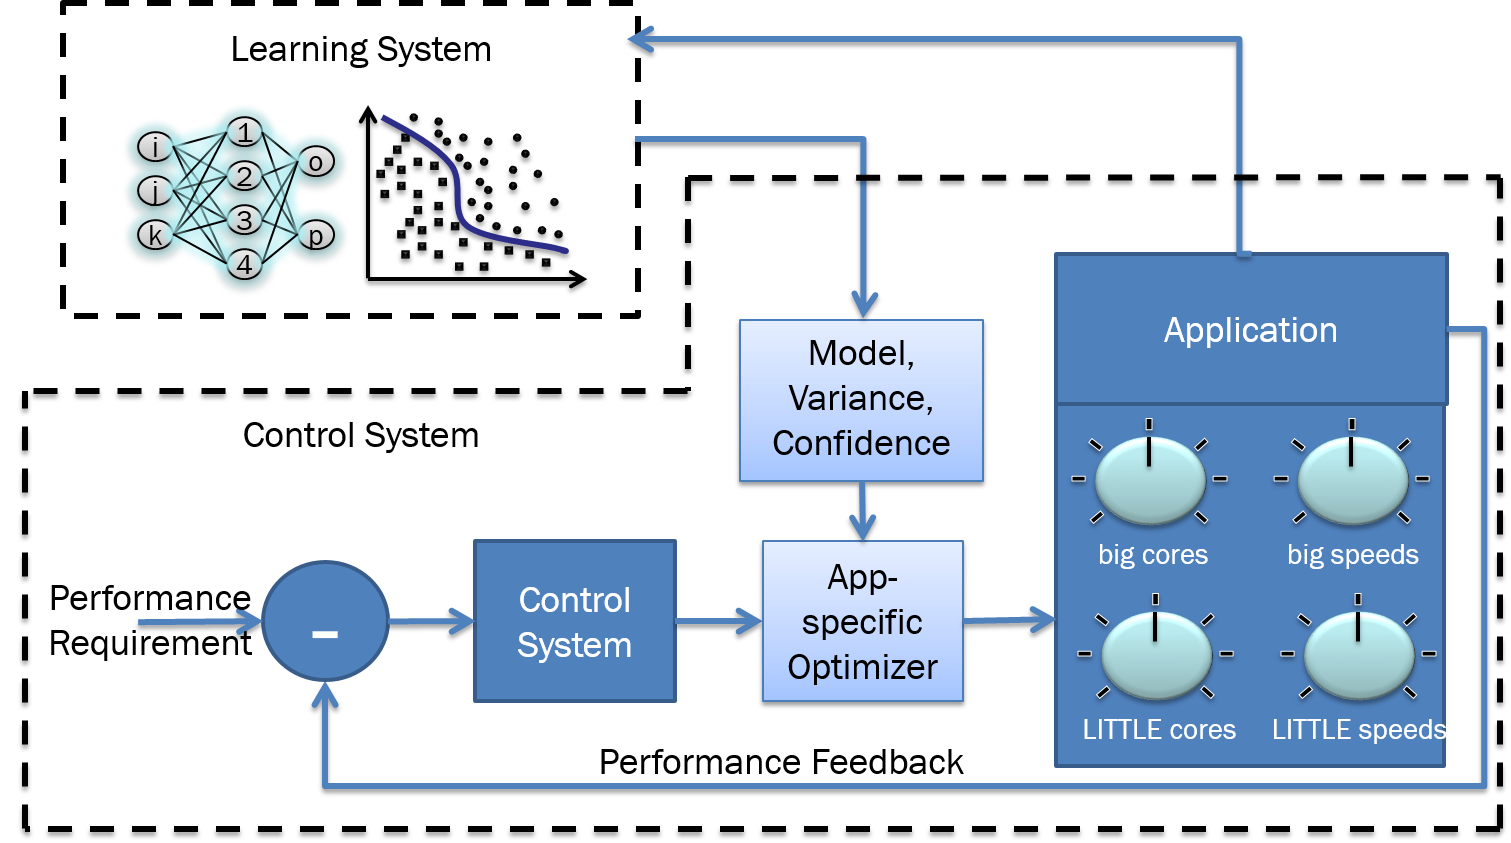
\includegraphics[width=\columnwidth]{figures/Overview.png}
  \caption{\SYSTEM{} overview.}
  \label{fig:overview}
\end{figure}


We describe \SYSTEM{}'s parmeter-free resource management system,
which assumes no prior knowledge of the application and requires no
user-specified parameters.  \figref{fig:overview} shows \SYSTEM{}'s
approach to this problem.  A generalized adaptive control system (GCS)
allocates resources to the new application to meet its specified
performance goal with minimal energy.  The GCS starts with a generic
resource model, allocates resources according to that model, and
records performance and power for a small number of configurations.
The recorded values are sent to a learning system, which estimates the
application's performance and power in all other configurations and
extracts those that represent Pareto-optimal tradeoffs in
performance/power.  These configurations are packaged in a special
data structure---the performance hash table (PHT).  The learner sends
the PHT, the estimated variance, and a confidence interval to the
control system.  Using these values, the GCS selects an energy minimal
resource configuration in constant time with formal guarnatees that it
will converge to the desired performance.

\begin{figure}
  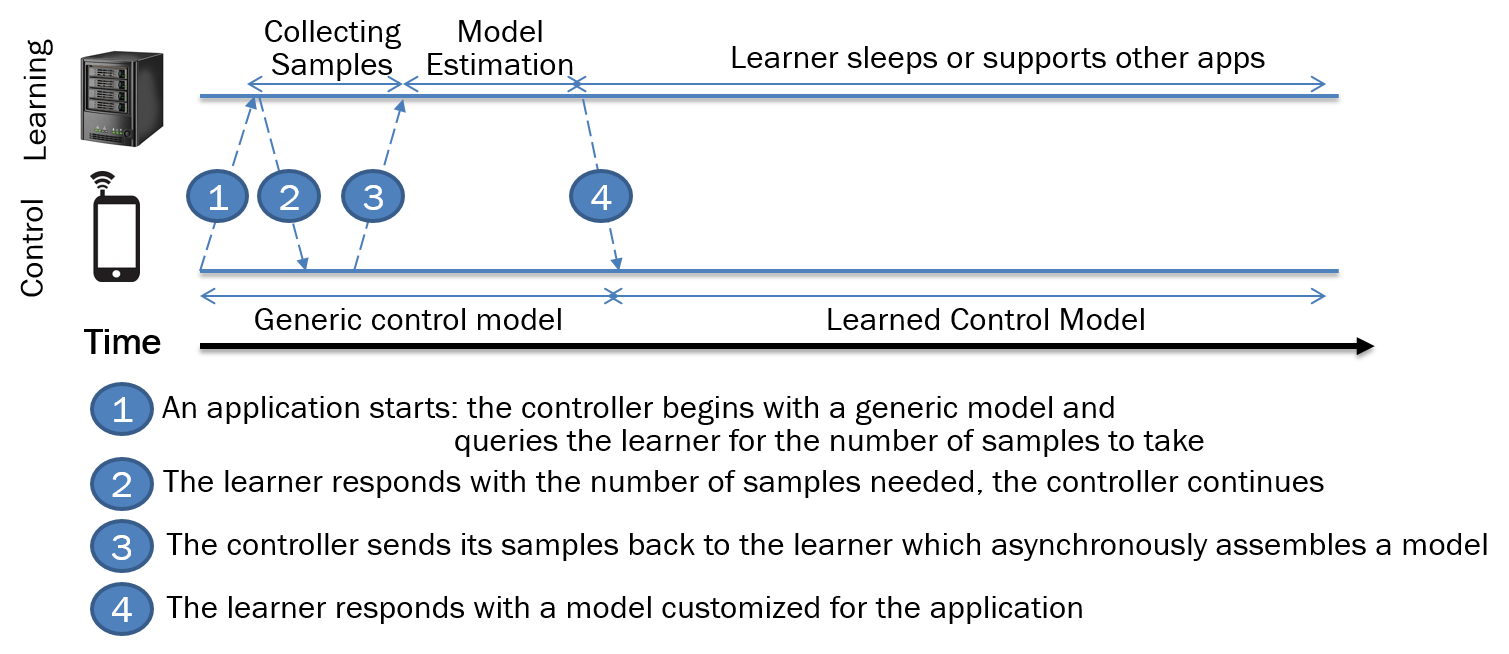
\includegraphics[width=\columnwidth]{figures/Timeline.png}
  \caption{Temporal relationship of the learning and control system.}
  \label{fig:timeline}
\end{figure}

\figref{fig:timeline} illustrates the asynchronous interaction between
\SYSTEM{}'s learning and control systems over time. The controller
starts when a new application launches with a performance goal.  Since
the controller has no prior knowledge of this application it starts
with a generic system model and allocates resources to the application
using this model.  At application launch, the controller sends a
message to the learner (message 1, in the figure) specifying the
application name and device type.  Based on the application and
device, the learner determines how many samples it needs for an
accurate estimate and sends this back to the controller (message 2).
The controller takes these samples during the course of applying the
generic model to determine resource configurations.  Once the correct
number of samples are measured, the controller sends the learner a
message with the performance and power of each measured configuration
(message 3).  Computationally expensive learners may require some time
to build a model from these observations.  Once the learner has a
model and variance estimate, that data is sent back to the controller
(message 4). From that point on, the controller uses this learned model.  

\figref{fig:timeline} shows several key points about the relationship
between learning and control.  First, the controller never waits for
the learner---it uses a generic model to provide less efficient
control until the learner can produce a customized model. Second, the
controller does not need to conintuously communicate with the learner,
this interaction happens once at application launch.  Third, if the
learner crashed, the controller would just default to the behavior of
a generic adaptive control system.  If the learner crashed after
producing a model, the control might not even need to know.  Finally,
because the learner and controller have a clearly defined interface,
they can be run in separate processes or even on physically separate
devices.

In the remainder of this section, we first describe a typical adaptive
control system would look like if designed for a heterogeneous
processor.  We then describe how we generalize this approach and
separate out parameters to be learned.  Next, we describe the general
class of learning systems that can work with this approach.  Then, we
describe how to encode the learned model so that it can be efficiently
accessed by the controller.  Finally, we discuss the formal guarantees
provided by the \SYSTEM{} approach.


\subsection{Traditional Control for Computing}
Several researchers have proposed techniques for controlling computing
systems.  A controller that can manage multiple resources to meet
multiple goals is known as a multiple-input, multiple-ouput (MIMO)
controller.  The inputs are measurements, \eg{} performance.  The
outputs are the resource settings to be used at a particular time,
\eg{} an allocation of big and LITTLE cores and a clockspeed for each.

The following difference equations describe a generic MIMO controller
for allocating $n$ resources to meet $m$ goals at time
$t$:\footnote{We assume discrete time, and thus, use diffference
  equations rather than differential equations that would be used for
  continuous systems.}
\begin{equation}
\begin{aligned}
&\x(t+1) &=& \mathbf{A} \cdot \x(t)& + \mathbf{B} \cdot \mathbf{c}(t)\\
&\y(t)   &=& \mathbf{C} \cdot \x(t)&
\end{aligned}
\label{eqn:system:mimo}
\end{equation}
Where $\x \in \R^{q}$ is the controller's \emph{state}, an abstract
representation of the relationship between resources.  $\mathbf{c}(t)
\in \R^n$ is a vector representing the current \emph{configuration} of
resources; \ie{} the $i$th vector element represents the amount of
resource $i$ to be allocated at time $t$.  $\y(t) \in \R^{m}$
represents the current value of the goal dimensions at time $t$. The
matrices $\mathbf{A} \in \R^{q \times n}$ and $\mathbf{B} \in \R{q
\times n}$ relate the resource configuration to the controller state.
The matrix $\mathbf{C}$ relates the controller state to the expected
behavior.  This model does not assume the states or the resources are
independent, but it does assume that their relationship is linear.  

For example, to allocate resources to meet performance goals in our
ARM big.LITTLE system---from \secref{example}---there are four
resources: the number of big cores, the number of LITTLE cores, and
the speeds for each of the big and LITTLE cores.  There is also a
single goal: performance.  Thus, in this example, $n=4$ and $m=1$.
The matrices $\mathbf{A}$, $\mathbf{B}$, and $\mathbf{C}$.  In this
example, we know there is a non-linear relationship between the
resources.  We can overcome this difficulty by tuning the identified
matrices at each time step---approximating the non-linear system
through a series of changing linear formulations.  This approximation
is a form of \emph{adaptive} or \emph{self-tuning} control
\cite{AdaptiveControl}.  Such adaptive controllers provide formal
guarantees that they will converge to the desired performance even in
the face of non-linearities, but they still assume convexity.

This control formulation has several drawbacks.  First, because it
requires matrix computation, its overhead scales linearly in the
number of resources \cite{Hellerstein2004a,METE}.  Second, the
adaptive mechanisms are not parameter-free---they require users to
specify starting values of the matrices $\mathbf{A}$, $\mathbf{B}$,
and $\mathbf{C}$ that account for any non-convexity in the
relationship between resources and
performance\cite{POET,METE,ControlWare,AdaptiveControl}.  Therefore,
typically 100s to 1000s of samples are taken when the controller is
designed to ensure that the starting matrices are sufficient to
prevent the controller from getting stuck in a local optima
\cite{FSE2015,sysid}.  Finally, these techniques cannot minimize
energy.  While \emph{optimal} control techniques exist, they find the
minimal change in resources that can meet the goal; \ie{} they cannot
minimize some other function of the resources, like energy consumption
\cite{josep-isca2016,Hellerstein2004a,optimal-control}.

\subsection{\SYSTEM{} Control System}
To overcome the above issues, \SYSTEM{} abstracts the controller of
\eqnref{system:mimo} and factors out those parameter that can be
estimated by a learner.  Specifically, \SYSTEM{} takes three steps to
transform a standard control system into one that can allocate
resources to meet a performance goal with minimal energy: 
\begin{enumerate}
\item controlling \emph{speedup} rather than directly controlling
  resources,
\item translating speedup into an energy
  minimal \emph{resource schedule}, and  
\item exploiting the \emph{problem structure} to solve it in constant
  time.  
\end{enumerate}
These steps assume a separate learner has produced a model of resource
performance and power.  The result is that \SYSTEM{}'s controller runs
in constant time without requiring any user-specified parameters.


% We first describe our formulation for controlling speedup and then
% converting that speedup into resource allocations.

\subsubsection{Controlling Speedup}
Instead of the matrix equations of \eqnref{system:mimo}, \SYSTEM{}
uses a scalar difference model relating speedup to performance:
\begin{equation}
  perf(t) = b \cdot speedup(t-1) + \delta \label{eqn:speedup}
\end{equation}
where $b$ is the application's \emph{base speed}: defined as the speed
when all resources are available.  While $b$ is application specific,
it is easy to measure online, by simply allocating all resources. Such
a configuration should not violate any performance constraints
(although it is unlikely to be energy efficient) so it is safe to take
this measurement.

With this model, \SYSTEM{}'s control law is simply:
\begin{eqnarray}
  error(t) &=& goal - perf(t) \label{eqn:speedup-error} \\
  % speedup(t) &=& speedup(t-1) - \frac{error(t)}{b}
  speedup(t) &=& speedup(t-1) - \frac{1 - \rho(t)}{b}.error(t)
  \label{eqn:speedup-control}
\end{eqnarray}
which states that the speedup at time $t$ is a function of the
previous speedup, the error at time $t$, the base speed $b$, and the
controller's \emph{pole} $rho(t)$.  Standard control techniques
statically determine the pole, but \SYSTEM{} \emph{dynamically sets
  the pole to account for error in the learned models---an essential
  modification for providing formal guarantees of the combined control
  and learning systems.}  For stable control, \SYSTEM{} ensures $ 0
\le $rho(t)$ < 1$. Small values of $\rho(t)$ eliminate error quickly,
but ma ke the controller more sensitive to model inaccuracies.  Larger
$\rho(t)$ makes the system more robust at the cost of reduced
convergence time.  We describe how \SYSTEM{} automatically sets the
pole in \secref{guarantees}.  First, however, we address the problem
of converting an abstract speedup into a resource allocation.

\subsubsection{Converting Speedup to Resource Schedules}
\SYSTEM{} must map \eqnref{speedup-control}'s speedup into a resource
allocation.  On our example ARM big.LITTLE architecture that means
mapping speedup into an allocation of big and LITTLE cores as well as
a speed for both (big and LITTLE cores are in separate clock domains).

The primary challenge is that speedups in real systems discrete
non-linear functions of resource usage, while \eqnref{speedup-control}
is a continuous linear function.  We bridge this divide by assigning
time to resource allocations such that the average speedup over a
control interval is that produced by \eqnref{speedup-control}.

We call an assignment of time to resources a schedule. There are
typically many schedules that meet a particular performance
requirement and we want to find a minimal energy schedule. Given a
time interval $T$, a speedup requirement $speedup(t)$ to average over
the time interval, and a configuration set of size $C$ , we formalize
this problem as:
\begin{eqnarray}
  \minimize_{\mathbf{\tau} \in \R^{C}} && \sum_{c=0}^{C-1} \tau_c \cdot p_c \label{eqn:power}  \\
  \st %&& \nonumber\\
  && \sum_{c=0}^{C-1} \tau_c \cdot s_c =  speedup(t)T \label{eqn:work} \\
  && \sum_{c=0}^{C-1} \tau_c =  T \label{eqn:deadline} \\
  && 0 \le \tau_c \le T, \qquad \forall c \in \{0,\ldots,C-1\} \label{eqn:time}
\end{eqnarray}
where $p_c$ and $s_c$ are configuration $c$'s estimated
\emph{powerup}---analogous to speedup---and speedup; $\tau_c$ is the
time to spend in configuration $c$.  \eqnref{power} states that the
objective is to minimize energy (power times time).  \eqnref{work}
states that the average speedup must be maintained, while
\eqnref{deadline} requires the time to be fully utilized.
\eqnref{time} simply avoids negative time.

\subsection{Exploiting Structure for Fast Solutions}
\SYSTEM{} now must solve \eqnrref{power}{time} on the local device
(see \figref{fig:timeline}, so the solution must be efficient.  By
expoiting the problem structure and encoding the learned model in the
performance hash table (PHT), \SYSTEM{} solves \eqnrref{power}{time}
in constant ($O(1)$) time.

Kim et al. analyze solutions to the problem of minimizing energy while
meeting a performance constraint \cite{kim-cpsna}.  They observe that
there must be an optimal solution with the following properties:
\begin{itemize}
\item At most two of $\tau_c$ are non-zero, meaning that at most two
  configurations will be used in any time interval.
\item If you chart the configurations in the power and performance
  tradeoff space the two configurations with non-zero $\tau_c$ lie on
  the lower convex hull of the power performance tradeoff space.
\end{itemize}
%\SYSTEM{} uses these two facts to construct a constant time algorithm
%for finding the optimal solution online.

\begin{figure}
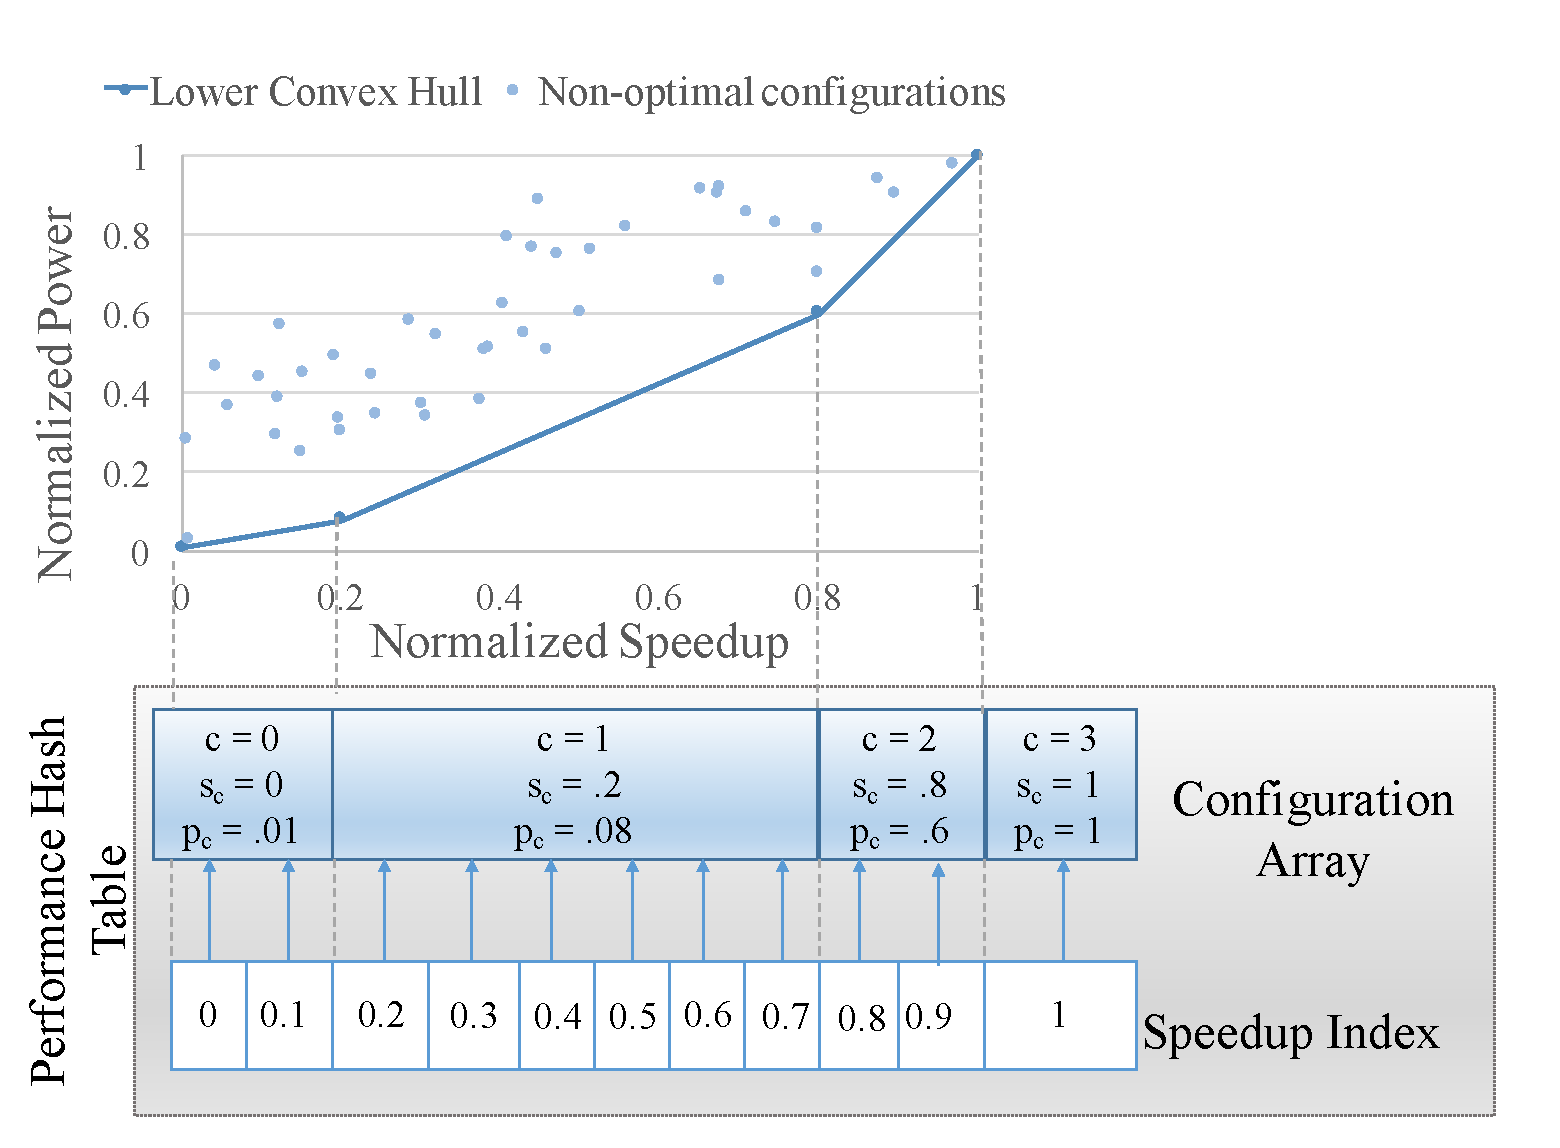
\includegraphics[width=\columnwidth]{figures/performance-hash-table.pdf}
\caption{Data structure to efficiently convert required speedup into a
  resource configuration.}
  \label{fig:pht}
\end{figure}

The PHT (shown in \figref{fig:pht}) only contains points on the lower
convex hull of the power/performance tradeoff space.  It consists of
two arrays: an array of pointers into a second array, which stores the
configurations on the lower convex hull sorted by speedup.  Recall
that speedups are computed relative to the base speed which uses all
resources.  The largest speedup is therefore 1, so SYSTEM{} needs only
consider speedups between 0 and 1.  The first table of pointers has a
\emph{resolution} indicating how many decimal points of precision it
captures.  The example in \figref{fig:pht} has a resolution of $0.1$.
Each pointer in the first table points to the configuration in the
second array that has the largest speedup less than or equal to the
index.

\SYSTEM{} computes $speedup(t)$ and uses the PHT to convert speedup
into two configurations referred to as $hi$ and $lo$.  To find the
$hi$ configuration, the translator clamps the desired speedup to the
largest index lower than $speedup(t)$ and then walks forward until it
finds the first configuration with a speedup higher than $speedup(t)$.
To find the $lo$ configuration, the translator clamps the desired
speedup to the smallest index higher than $speedup(t)$ and then walks
backwards until it finds the configuration with the largest speedup
less than $speedup(t)$.

For example, consider the PHT in \figref{fig:pht} and an optimizer
meeting $speedup(t) = .65$.  To find $hi$, the optimizer indexes at .6
and walks up to find $c=2$ with $s_c=.8$, setting $hi = 2$.  To find
$lo$, the optimizer indexes the table at .7 and walks backward to find
$c=1$ with $s_c=.2$, setting $lo = 1$.

Finally, \SYSTEM{} sets $\tau_{hi}$ and $\tau_{lo}$ by solving the
following set of equations:
\begin{eqnarray}
  T &=& \tau_{hi} + \tau_{lo}    \label{eqn:s1} \\
  speedup(t) &=& \frac{s_{hi} \cdot \tau_{hi} + s_{lo} \cdot \tau_{lo}}{T} \label{eqn:s2}
\end{eqnarray}
In these equations, $speedup(t)$ is the speedup requested by the
controller and $s_c$ are speedups estimated by the learner.  By
solving \eqnsref{s1}{s2}, \SYSTEM{} has turned the controller's
speedup into a schedule of resource allocations using learned models
of speedup and powerup.

\subsection{\SYSTEM{} Learning Requirements}
The previous subsection describes a general control system, which can
be customized with a number of different learning methods.  The
requirements on the learner are 1) that it must produce estimates of
the speedup and powerup values stored in the PHT and 2) that it
produce an estimate of its own inaccuracy.  This section describes the
general class of learning mechanisms that meet these requirements.

\TODO{Fill in.}


\subsection{Formal Analysis}
\subsubsection{Control System Complexity}
%\subsubsection{Algorithmic Analysis}

\SYSTEM{}'s control system (see Algorithm \ref{alg:gcs}) runs on the
local device along with the application under control, so its overhead
must be minimal.  In fact, each controller invocation is $O(1)$ .  The
only part that is not obviously constant time is the PHT lookups.
Provided the PHT resolution is sufficiently high to avoid collisions,
then each PHT lookup requires constant time.
\begin{algorithm}[t]
\caption{Generalized control system}
\label{alg:gcs}
\begin{algorithmic}
\REQUIRE Initialize the controller with a general model of speedup and powerup. Send power and performance samples to server and get performance hash table(PHT) from the server.
\WHILE{$True$}
    \STATE    Measure streaming application performance 
    \STATE    Compute required speedup (Equation \eqref{eqn:speedup})
    \STATE    Lookup $s_{hi}$ and $s_{lo}$ with PHT
    \STATE    Compute $\tau_{hi}$ and $\tau_{lo}$ (Equations \ref{eqn:s1} \& \ref{eqn:s2})
    \STATE    Configure to system to $hi$ $\&$ sleep $\tau_hi$.
    \STATE    Configure to $lo$ $\&$ sleep $\tau_lo$.
\ENDWHILE
\vskip -1.5em
\end{algorithmic}
\end{algorithm}

\subsubsection{Control Theoretic Formal Guarantees}
\label{sec:guarantees}
As mention above, the pole $\rho(t)$ is critical to provide control
theoretic quarantees in the presence of learned models.  \SYSTEM{}
requires that any learner estimate not only speedup and powerup, but
also the variance $\sigma$.  \SYSTEM{} uses that information to derive
a lower bound for the pole which guarantees probabilistic convergence
to the desired performance. Specifically, we prove that with
probability 99.7\% the system will converge to the desired performance
if the pole is set to,
$$\Floor{1- \Floor{max(\hat{s})/(min(\hat{s}) - 3\sigma)}_0}_0 \leq \rho(t)
< 1,$$ where $\Floor{x}_0 = \max(x,0)$ and $\hat{s}$ is the
estimated speedup. We include the proof of this claim in the appendix. In principle, users who need higher confidence
could set the scalar multiplier on $\sigma$ higher, using $6$ for
example provides a 99.99966\% probability of convergence.  

Thus we provide a lower-bound on the value of $\rho(t)$ required for a
user to be confident that \SYSTEM{} will converge to the desired
performance.  This value for the pole only considers performance, and
not energy efficiency.  In practice, we find that it is often better
to use a higher pole based on the \emph{uncertainty} between the
controller's observed energy efficiency and that predicted by the
model.  We follow prior work in quantifying uncertainty as $\rho(t) $
\cite{Tokic2010}:
\begin{equation}
  \begin{array}{rcl}
    \beta(t) &=&  \text{exp}{\left(- \left( \left|   \frac{\bar{s}(t)}{\bar{p}(t)}  -\frac{ \hat{s}(t)}{\hat{p}_(t)} \right| \right) /5\right)} \\
    \rho(t) &=& \frac{1-\beta(t)}{1+\beta(t)} 
  \end{array}
  \label{eqn:uncer}
\end{equation}
where $\bar{s}$ and $\bar{p}$ are the measured values of speedup and
power up and $\hat{s}$ and $\hat{p}$ are the estimated values from the
learner.  This measure of uncertainty captures both power and
performance.  We find that it is generally higher than the pole value
given by our lower bound, so in practice we set the pole dynamically
to be the higher of the two values and we allow \SYSTEM{} to make spot
updates to the estimated speedup and power based on its observations.
